\documentclass{article}
\usepackage{indentfirst}
\usepackage{lmodern}
\usepackage[utf8]{inputenc}
\usepackage[T1]{fontenc}
\usepackage[ngerman]{babel}
\usepackage{amssymb,amstext,amsmath}
\usepackage{graphicx}
\usepackage{dsfont}
\usepackage{amsfonts}
\usepackage{graphics}
\usepackage{float}
\usepackage{cite}
\usepackage{url}
\usepackage{tabularx}
\usepackage{capt-of}

\title{Schallwellen}
\author{Alexander Heinisch, Dominik Wille}
\begin{document}
\maketitle

{\begin{center}
\begin{minipage}{\linewidth}
\centering
\makebox[0cm]{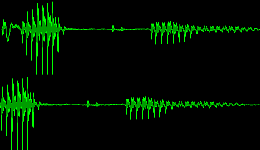
\includegraphics[width=7cm]{bilder/sal0}}
\label{wtd}
\end{minipage}
\end{center}

\vspace{7cm}
\noindent
\begin{center}
\begin{tabular}{r l}
Tutor & Brünig\\
Durchführung & 12. Juni 2013 von 14-18 Uhr \\

E-Mail Dominik & dominik.wille@fu-berlin.de \\
E-Mail Alexander & Matthias.Heinisch@gmx.de \\
\end{tabular}
\end{center}

\newpage
\tableofcontents
\newpage

\section{Physikalische Grundlagen}
\subsection{Schallwellen und Ausbreitungsgeschwindigkeit}
Tritt eine zunächst lokale Erregung in einem ausgedehnten, elastischen Medium auf, entsteht eine Welle, welche sich räumlich ausbreitet. Die Geschwindigkeit, mit der sich diese Erregung ausdehnt, nennt man Phasen-, bzw. Schallgeschwindigkeit und hängt von der Rückstellkraft und der Trägheit des Mediums ab. Es gilt:

\begin{equation}
\label{c}
c=\sqrt{\frac{D}{\rho}}
\end{equation}

Mit der Rückstellkonstanten D und der Dichte \(\rho\).\\
Nimmt man nun einen Festkörper als Medium, besitzt in diesem jedes Volumenelement eine fest definierte Ruheposition. Nun unterscheidet man zwischen zwei Arten von Wellen in diesem Körper. Die Erste ist die longitudinale Dichtewelle, welche in Ausbreitungsrichtung schwingt. Des Weiteren gibt es die transversale Scherwelle. Sie schwingt im Gegensatz zur Longitudinalwelle senkrecht zur Ausbreitungsrichtung, ist nicht an ein Medium gebunden und kann polarisiert werden (z.B. Licht).In Gasen und Flüssigkeiten treten nur Dichtewellen auf, wodurch die Rückstellkonstante durch das Kompressionsmodul K ausgedrückt wird.\\
Da zum einen die Periodendauer von Schallwellen in Gasen relativ kurz ist, und zum anderen Gase eine geringe Wärmeleitfähigkeit besitzen, findet kein Energieaustausch zwischen den einzelnen Teilchen statt. Damit gilt die Poisson-Gleichung:

\begin{equation}
\label{rho}
\rho \cdot V^{\kappa} = const.
\end{equation}

welche durch Ableiten einen Ausdruck für die Kompressionsrate K liefert:

\begin{equation}
\label{K}
D = K = V \frac{d\rho}{dV}=-\kappa \rho
\end{equation}

mit dem Isentropenindex 

\begin{equation}
\label{kappa}
\kappa = \frac{c_{p}}{c_{v}}
\end{equation}

Daraus folgt für c:

\begin{equation}
c=\sqrt{\kappa\frac{p}{\rho}}=c(T)
\end{equation}

Die Schallgeschwindigkeit ist wegen der Dichte Temperaturabhängig, wobei sie nicht Druckabhängig ist, da sich die Trägheits- und Rückstellgröße im gleichen Maße mit dem Druck ändert.

\newpage
\subsection{Stehende Welle}
Durch Reflexion und Interferenz an den Grenzen eines beschränkten Volumens, entsteht eine Folge stationärer Schwingungszustände.Es bildet sich also eine stehende Welle, wenn die Wellenlänge \(\lambda\) in einem bestimmten Verhältnis zur Resonatorlänge \(l\) steht.\\
Ist der Resonator nun einseitig abgeschlossen, gilt die Relation:

\begin{equation}
\label{l1}
l=\left(n-\frac{1}{2}\right)\frac{\lambda}{2}
\end{equation}

Im beidseitig abgeschlossenen Fall, gilt:

\begin{equation}
l=n\cdot\frac{\lambda}{2}
\end{equation}

In der folgenden Abbildung werden diese Formeln noch einmal graphisch dargestellt.
{\begin{center}
\begin{minipage}{\linewidth}
\centering
\makebox[0cm]{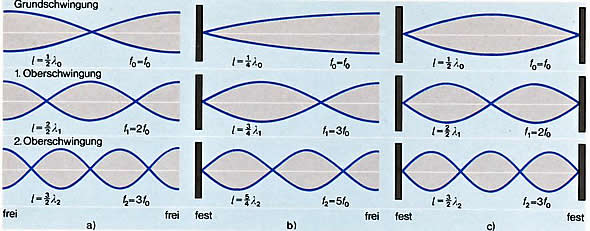
\includegraphics[width=\textwidth]{bilder/sal1}}
\captionof{figure}{Darstellung von Wellen in a) unbegrenzten Medien, b) einseitig abgeschlossenem Resonator, c) und beidseitig abgeschlossenem Resonator}
\label{welle}
\end{minipage}
\end{center}

Kennen wir nun die Wellenlänge und die Frequenz , ergibt sich daraus die Fundamentalbeziehung der Schallgeschwindigkeit aus:

\begin{equation}
c=\lambda\cdot f
\end{equation}

Im Versuch werden wir bei der Untersuchung einer Gassäule in einem Rohr nur Longitudinalwellen beobachten. Befestigen wir den Stab in der Mitte, wird an einem Ende ein Phasensprung von \(\pi\) auftreten und man kann die Grundschwingung von n=1 beobachten.\\
Befindet sich der Stab hingegen zu einem viertel seiner Länge vom Rand entfernt, ist die ''erste Harmonische'' mit n=2 zu beobachten.\\


\newpage
\section{Aufgaben}
\subsection{Aufgabe 1}
Messung der Schallgeschwindigkeit in Luft durch Laufzeitmessung.
\subsection{Aufgabe 2}
Beobachtung der Resonanzen einer Luftsäule mit abgeschlossenem bzw. offenem Ende durch Variation der Anregungsfrequenz. Berechnung der Schallgeschwindigkeit und des Verhältnisses der spezifischen Wärme \(\frac{c_{p}}{c_{v}}=\kappa\) von Luft (Isentropenindex, Adiabatenkoeffizient).
\subsection{Aufgabe 3}
Bestimmung der Schallgeschwindigkeit in Metallen aus der Laufzeit bzw. der Grundschwingungsfrequenz für zwei verschiedene Einspannungen des Stabes. Berechnung des Elastizitätsmoduls des Metalls.
\subsection{Ergänzende Frage}
Warum werden höhere Frequenzen stärker gedämpft als niedrige?

\newpage

\section{Auswertung}
\newpage
\section{Exercise 1}
In this task the oscillator will be deflected by hand to an amplitude near the maximum. The position resp. Angular of the flywheel Is measured and plotted with CASSY-Lab. 
\subsection{Observation}
The measured curves fit nearly perfectly the expectations of a exponential decreasing sin function. To process the data The envelope function will is fitted with a \(f(x)=A*e^{-x/B}+C\) function. The frequency  is measured just by counting the periods per time interval.
\subsection{Errors}
The equipment does not provide data which is totally free of systematic errors. There is a lot of friction which is not only dependent on the wheels velocity. But the systematic errors are not so significant that the data can not be evaluated.

It is assumed that the time is measured relatively correct \(\Delta t = 0.01\, s\). 
\subsection{Measured Data}
\begin{center}
\begin{tabular}{c|cccc}
Position & \(B [s]\) & \(N [1]\) & \(t_1 [s]\) & \(t_2 [s]\) \\ \hline
3 & \(5.12\) & \(6\) & \(1.72 \pm 0.001\) & \(13.6 \pm 0.001\) \\ 
3 & \(5.1\) & \(6\) & \(1.69 \pm 0.001\) & \(13.68 \pm 0.001\) \\ 
3 & \(5.13\) & \(6\) & \(1.65 \pm 0.001\) & \(13.62 \pm 0.001\) \\ 
2 & \(5.41\) & \(6\) & \(13.90 \pm 0.001\) & \(1.68 \pm 0.001\) \\ 
2 & \(5.34\) & \(6\) & \(1.70 \pm 0.001\) & \(13.92 \pm 0.001\) \\ 
2 & \(5.4\) & \(6\) & \(1.73 \pm 0.001\) & \(13.94 \pm 0.001\) \\ 
1 & \(27.13\) & \(20\) & \(42.01 \pm 0.001\) & \(4.22 \pm 0.001\) \\ 
1 & \(26.95\) & \(20\) & \(4.26 \pm 0.001\) & \(42.13 \pm 0.001\) \\ 
1 & \(27.23\) & \(20\) & \(14.83 \pm 0.001\) & \(52.64 \pm 0.001\) \\ 
0 & \(69.13\) & \(20\) & \(50.82 \pm 0.001\) & \(13.16 \pm 0.001\) \\ 
0 & \(68.89\) & \(20\) & \(13.08 \pm 0.001\) & \(50.73 \pm 0.001\) \\ 
0 & \(69.23\) & \(20\) & \(13,00 \pm 0.001\) & \(50.65 \pm 0.001\) \\ 
\end{tabular}
\captionof{table}{measured values for free damped oscillations}
\end{center}
\newpage
\subsection{Evaluation}
To determine the damping constant \(\delta\) the formula \eqref{x(t)_1} can be compared to the fitting function \(f(x)=A*e^{-x/B}+C\) and gives:
\begin{align}
\delta = \frac{1}{B}
\end{align}
Since \(\omega_1\) is determined as \(\omega_1 = \frac{N}{\left| t_1 - t_2 \right|}\) the eigenfrequency \(\omega_0\) can be determined with \eqref{w1} as:
\begin{align}
\omega_0 = \sqrt{\omega_1^2 + \delta^2}
\end{align}
All in all that means:
\begin{center}
\begin{tabular}{c|cccc}
Position & \(B\, [s]\) & \(\delta\, [\frac{1}{s}]\) & \(w_1\, [\frac{1}{s}]\) & \(w_0\, [\frac{1}{s}]\) \\\hline
3 & \(5.12\) & \(0.1953125\) & \(0.505050505050505\) & \(0.541500678954348\) \\ 
3 & \(5.10\) & \(0.196078431372549\) & \(0.500417014178482\) & \(0.537460639794978\) \\ 
3 & \(5.13\) & \(0.194931773879142\) & \(0.50125313283208\) & \(0.537822554047006\) \\ 
2 & \(5.41\) & \(0.184842883548983\) & \(0.490998363338789\) & \(0.524639194494724\) \\ 
2 & \(5.34\) & \(0.187265917602996\) & \(0.490998363338789\) & \(0.525497779916396\) \\ 
2 & \(5.40\) & \(0.185185185185185\) & \(0.491400491400491\) & \(0.52513616877979\) \\ 
1 & \(27.13\) & \(0.036859565057132\) & \(0.529380624669137\) & \(0.530662296862408\) \\ 
1 & \(26.95\) & \(0.037105751391466\) & \(0.528122524425667\) & \(0.529424439927044\) \\ 
1 & \(27.23\) & \(0.036724201248623\) & \(0.528960592435863\) & \(0.530233887362406\) \\ 
0 & \(69.13\) & \(0.014465499783018\) & \(0.531067445565587\) & \(0.531264418555892\) \\ 
0 & \(68.89\) & \(0.014515894904921\) & \(0.531208499335989\) & \(0.531406794246822\) \\ 
0 & \(69.23\) & \(0.014444604940055\) & \(0.531208499335989\) & \(0.531404851670238\) \\
\end{tabular}
\end{center}
To get a final value for the damping constants, the average value is used:
\begin{align}
\delta = \frac{\sum_{i=0}^n \delta_i}{n}
\end{align}
The error of the final damping constants is determined by the variance of the values:
\begin{align}
\Delta\delta &= \sqrt{\frac{\sum_{i=0}^n \left( \bar{\delta} -\delta_i\right)^2 }{n-1}}
\end{align}
The result is:
\begin{center}
\begin{tabular}{ccc}
\(\delta_0\) & \(=\) &\(\left(0.014475 \pm 0.000037 \right)\)\\
\(\delta_1\) & \(=\) &\(\left(0.03690 \pm 0.00019 \right)\)\\
\(\delta_2\) & \(=\) &\(\left(0.1858 \pm 0.0013 \right)\)\\
\(\delta_3\) & \(=\) &\(\left(0.19544 \pm 0.00058 \right)\)
\end{tabular}
\end{center}
The final eigenfrequency \(\omega_0\) is determined as the average value of the single eigenfrequencies:
\begin{align}
\omega_0 &= \frac{\sum_{i=0}^n \omega_{0_i}}{n} = 0.5314 \, \frac{1}{s}\\
\Delta \omega_0 &= \sqrt{\frac{\sum_{i=0}^n \left( \omega_0 -\omega_{0_i}\right)^2 }{n-1}} = 0.0053\, \frac{1}{s}
\end{align}
\end{document}